\section{Mechanics}
\label{sec:dp-pds-mechanics}

\subsection{\dshort{pmt} Support Structure}
\label{subsec:dp-pds-mechanics-pmtsupport}

A uniform array of \dpnumpmtch cryogenic Hamamatsu R5912-MOD20 \dwords{pmt}, below the transparent cathode structure, is fixed on the membrane floor in the areas between the membrane corrugations. The arrangement of the \dwords{pmt} accommodates the cryogenic piping on the membrane floor, and other elements installed in this area.

\begin{dunefigure}[Cryogenic Hamamatsu R5912-MOD20 \dword{pmt} fixed on the membrane floor.]{fig:dppd_3_2}
{Cryogenic Hamamatsu R5912-MOD20 \dword{pmt} fixed on the membrane floor, with the optical fiber of the calibration system.}
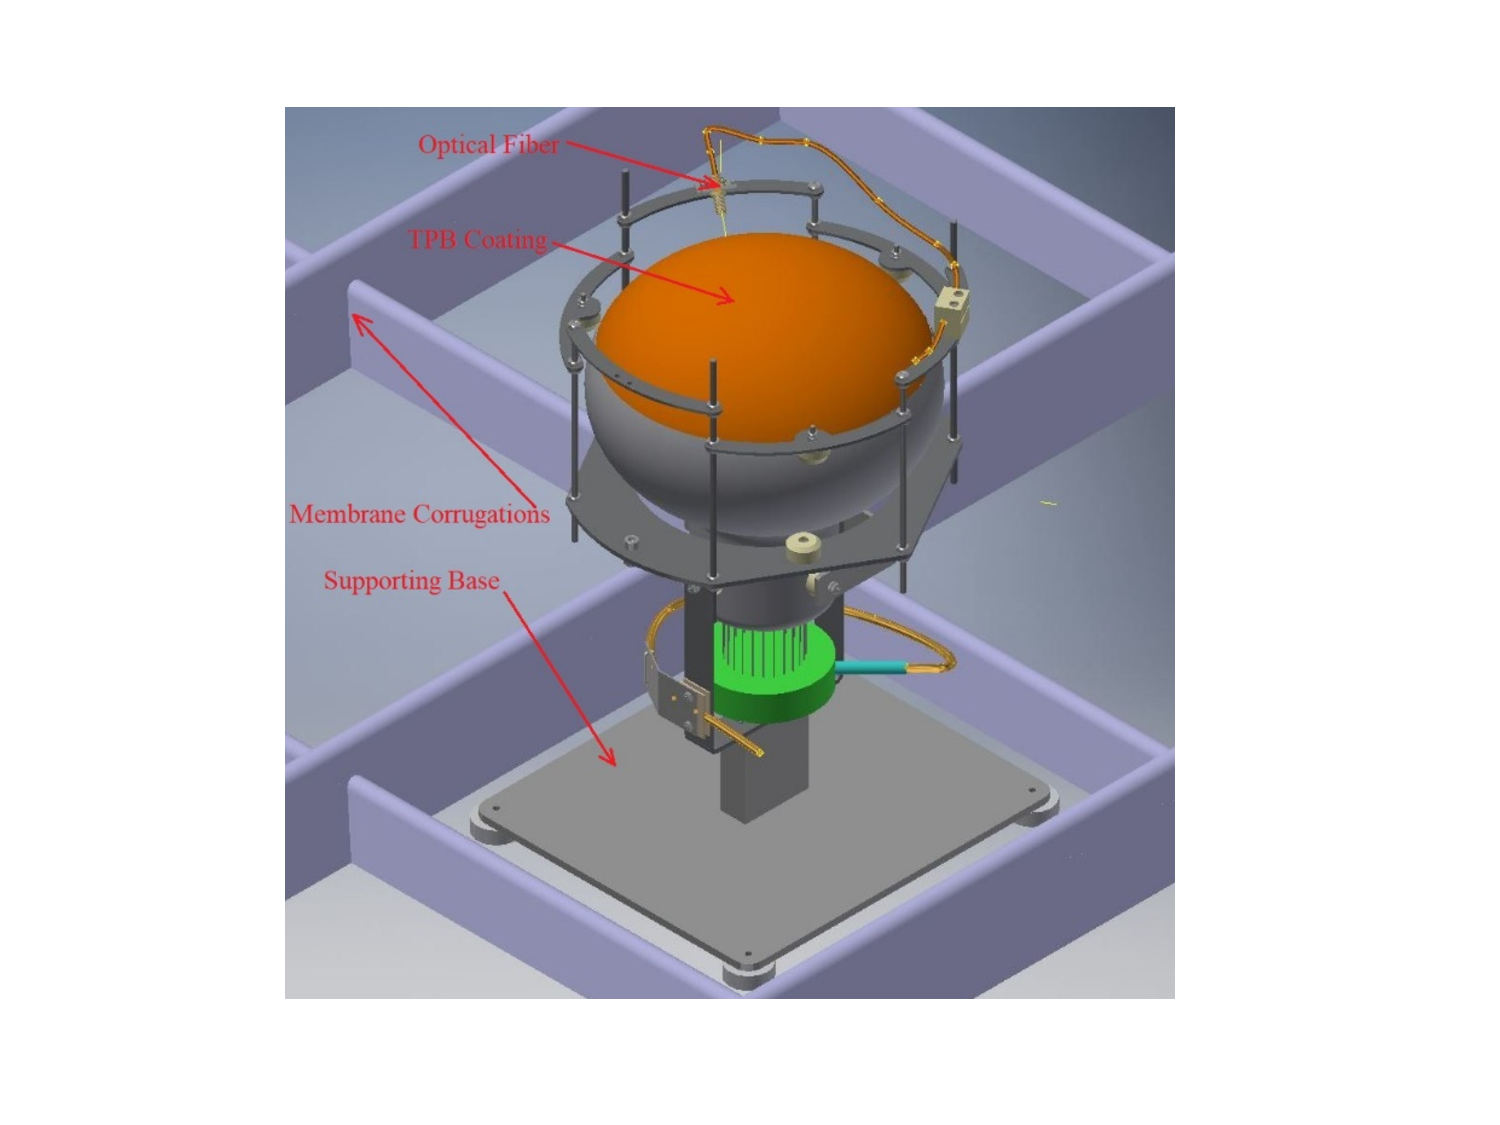
\includegraphics[width=0.42\textwidth]{dppd_3_2}
\end{dunefigure}

The mechanics for the attachment of the \dwords{pmt} has been carefully studied. It must counteract the \dword{pmt} buoyancy while avoiding stress to the \dword{pmt} glass due to differentials in the thermal contraction between the support and the \dword{pmt} itself. The attachment is done via a stainless steel supporting base that is point-glued to the membrane via four adhesive injection holes. The weight of the support and \dword{pmt} exceeds the buoyancy force of the system. Given the large standing surface of the stainless steel plate support basis, these supports also ensure stability against possible lateral forces acting on the \dwords{pmt} due to the liquid flow. Figure \ref{fig:dppd_3_2} depicts the \dword{pmt} together with its support base attached to the bottom of the cryostat.

As an alternative to the table-like assembly of the ground grid, the concept of individual ground grids for each \dword{pmt} is under study by \dword{hv} and \dual \dword{pds} consortia. In this option, the grids will be mechanically attached to the support structure. This will increase the acceptance of the \dwords{pmt} at larger angles.

The support frame structure is mainly composed of \num{304}L stainless steel with some small Teflon (PTFE) pieces assembled by A4 stainless steel screws that minimize the mass while ensuring the \dword{pmt} support to the cryostat membrane. The design %was done taking 
takes into account the shrinking of the different materials during the cooling process so as to avoid breaking of the \dword{pmt} glass.
Over-pressure tests were carried out for \dword{pddp}, and further tests to ensure the correct performance under pressure will be carried out. An individual \dword{pmt} mount has been designed and tested in the  \dword{wa105} prototype~\cite{Zambelli:2017dkg} and the same design is used for \dword{pddp}.

%%%%%%%%%%%%%%%%%%%%%%%%%%%%%%%%%%%%%%%%%%%%%%%%%%%%%%%%%%%%%%%%%%%%

\subsection{\dshort{wls} Reflector Foils}
\label{subsec:dp-pds-mechanics-foils}

\fixme{Add description here for foils on field cage walls for 2nd draft if included in baseline design. Otherwise, describe this in appendix.}